\documentclass{standalone}
\usepackage{tikz}
\usepackage{pgfplots}
\pgfplotsset{width=32cm,height=18cm,compat=1.3}
\pgfplotsset{every tick label/.append style={font=\Huge}}
\usepackage{filecontents}

\usetikzlibrary{patterns}

\definecolor{citrine}{rgb}{0.89, 0.82, 0.04}
\definecolor{arylideyellow}{rgb}{0.91, 0.84, 0.42}
\definecolor{bronze}{rgb}{0.8, 0.5, 0.2}

\begin{document}
	\centering
		\vspace{1.5em}
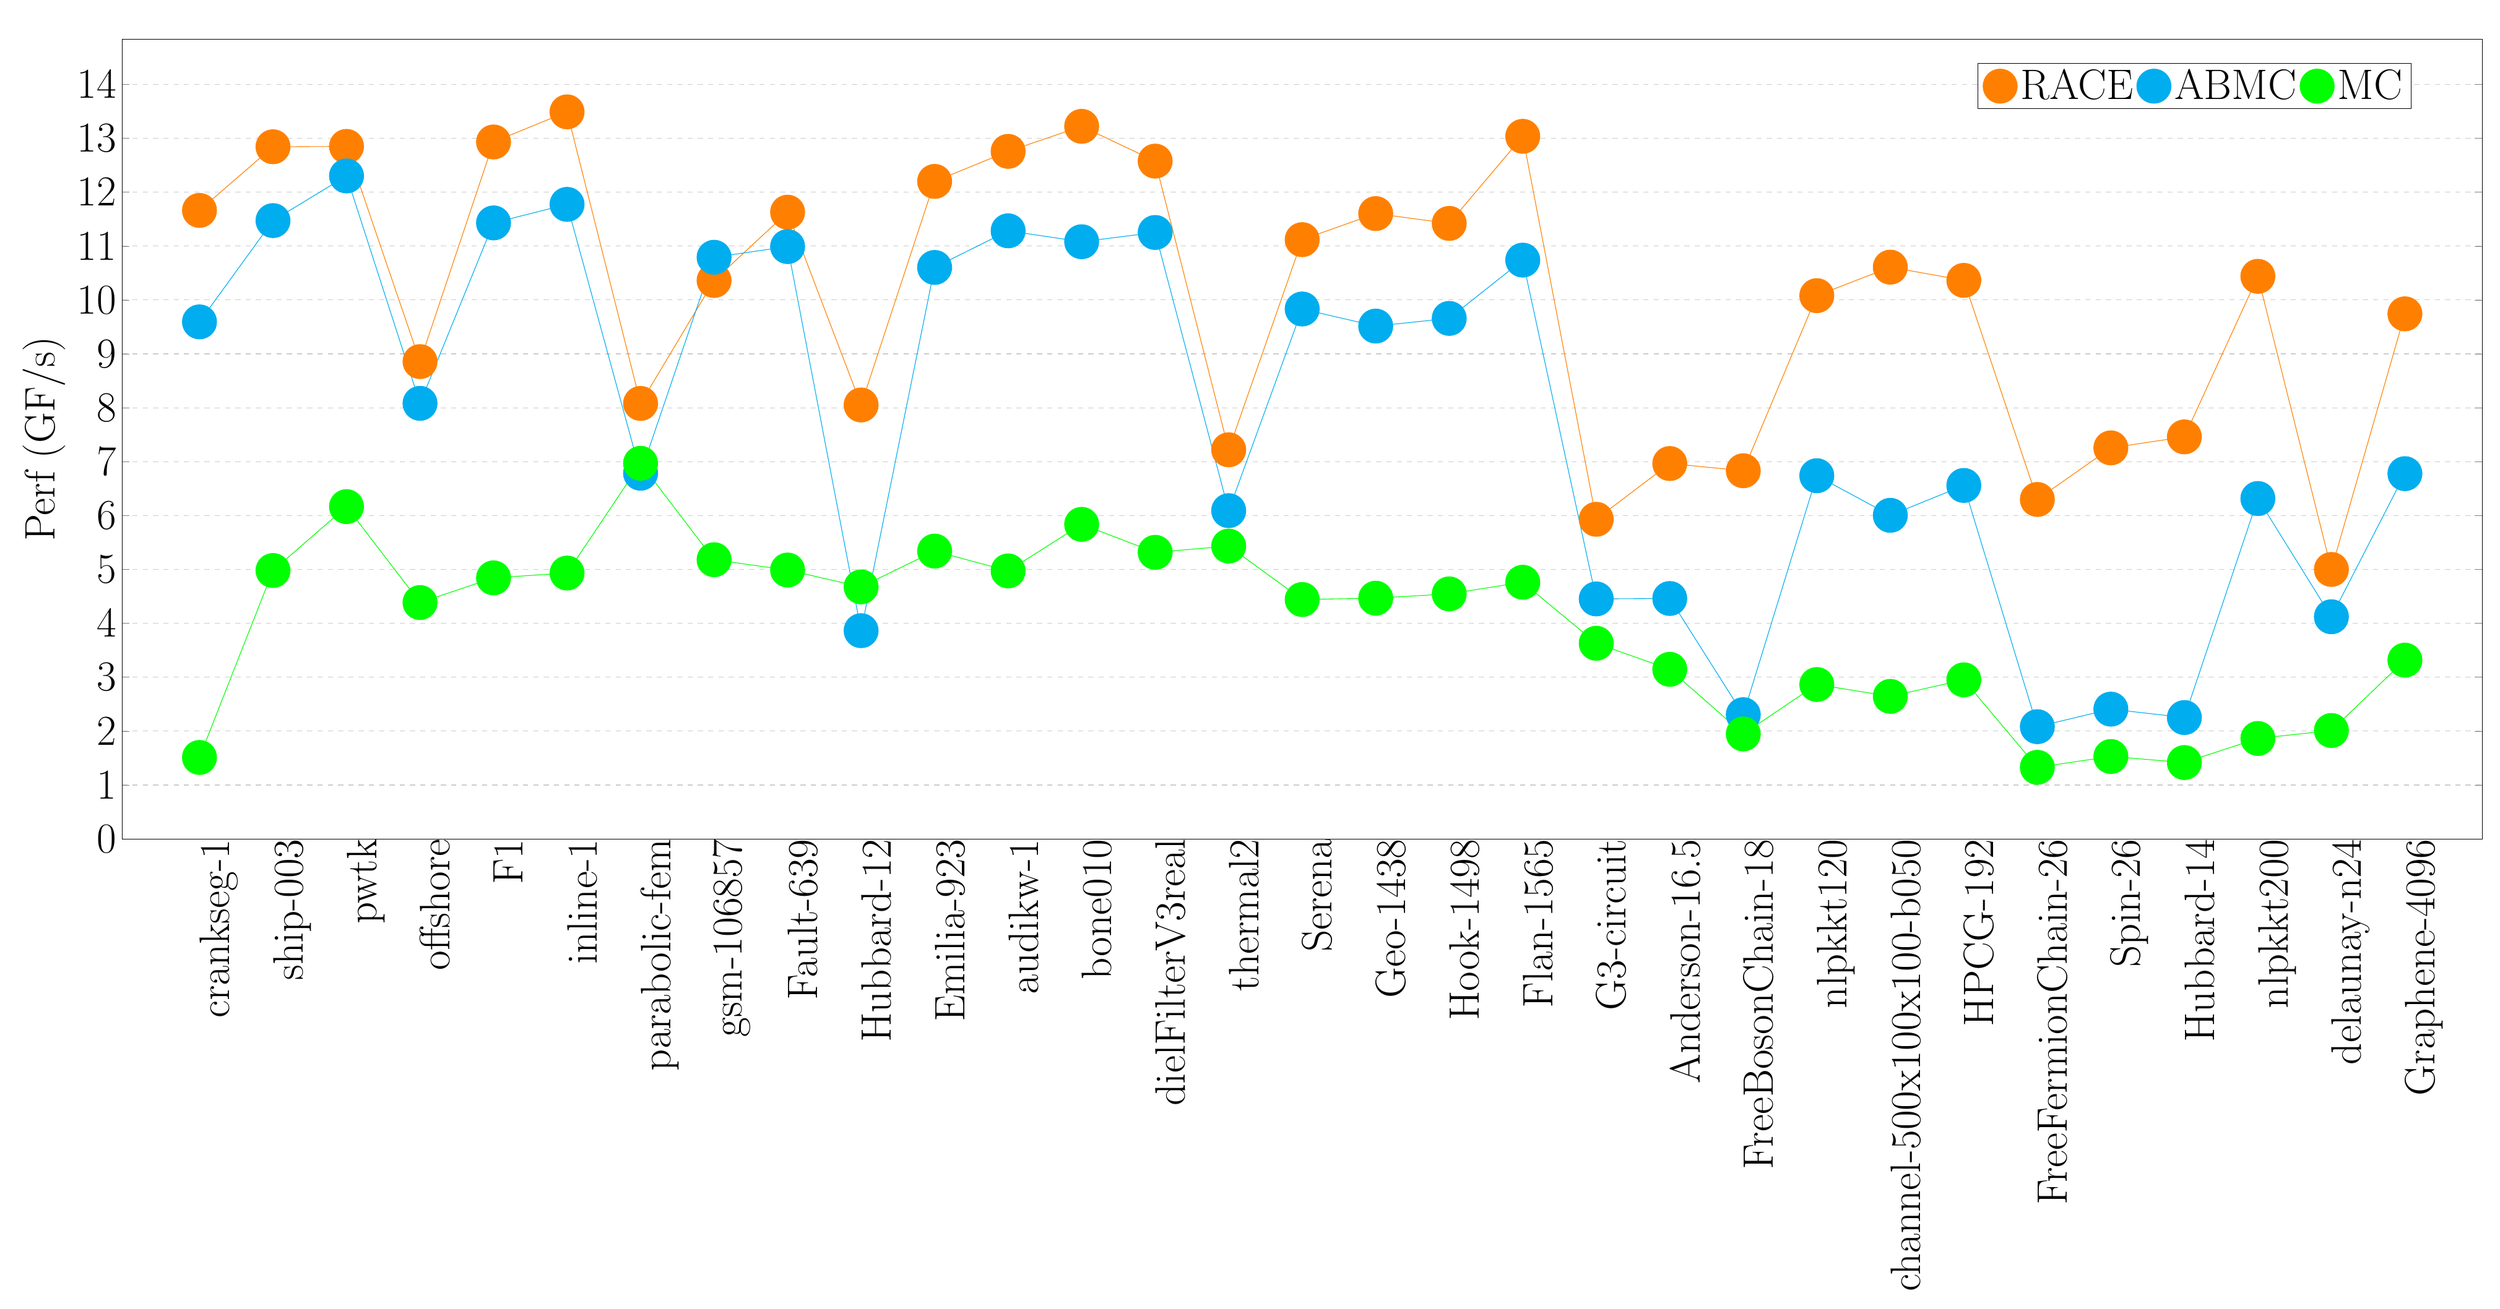
\begin{tikzpicture}
		%	\node at (13.25,15) {\LARGE{}};
			\begin{axis}[
		%	xmin=0.25, xmax=7.25,
			ymin=0, %ymax=3.25,
			xtick={1, 2, 3, 4, 5, 6, 7, 8, 9, 10, 11, 12, 13, 14, 15, 16, 17, 18, 19, 20, 21, 22, 23, 24, 25, 26, 27, 28, 29, 30, 31},
		%	ytick={0,0.5,1,1.5,2,2.5,3},
			xticklabels={crankseg-1, ship-003, pwtk, offshore, F1, inline-1, parabolic-fem, gsm-106857, Fault-639, Hubbard-12, Emilia-923, audikw-1, bone010, dielFilterV3real, thermal2, Serena, Geo-1438, Hook-1498, Flan-1565, G3-circuit, Anderson-16.5, FreeBosonChain-18, nlpkkt120, channel-500x100x100-b050, HPCG-192, FreeFermionChain-26, Spin-26, Hubbard-14, nlpkkt200, delaunay-n24, Graphene-4096},
			width  = 50cm,
			height = 18cm,
			major x tick style = transparent,
			%	minor ytick={1, 5, 10, 15, 20, 25, 30 ,35,40},
			grid = minor,	
			%add_bar_commands
			ymajorgrids = true,
			grid style={dashed, gray!40},
			ylabel = {\Huge{Perf (GF/s)}},
		%	symbolic x coords={Graphene-2048-2048, Graphene-4096-4096, Spin-24-24-24},
			x tick label style={rotate=90, anchor=north east, inner sep=0mm, font={\Huge}},
			tick label style={font={\Huge}},
			scaled y ticks = false,
			enlarge x limits=0.035,
			legend cell align=left,
			legend style={font=\Huge},
			legend columns=-1,
			legend style={
				%at={(1,1.05)},
				%anchor=south east,
				%column sep=1ex,
				legend pos=north east
			},
			%spl_legend_code
			title= {\Huge\scalebox{1.5}{{}}}
			]

\addplot[ mark=*, mark size=10pt, mark options={orange}, draw=orange ] plot coordinates{(1,11.661889) (2,12.843037) (3,12.849712) (4,8.856331) (5,12.932172) (6,13.490943) (7,8.080436) (8,10.361301) (9,11.629001) (10,8.051711) (11,12.200132) (12,12.757774) (13,13.222356) (14,12.576653) (15,7.219646) (16,11.119455) (17,11.603120) (18,11.420717) (19,13.037058) (20,5.930575) (21,6.965104) (22,6.831253) (23,10.080070) (24,10.609130) (25,10.363803) (26,6.298190) (27,7.255795) (28,7.459718) (29,10.439037) (30,4.999955) (31,9.742837)};
\addplot[ mark=*, mark size=10pt, mark options={cyan}, draw=cyan ] plot coordinates{(1,9.593575) (2,11.473052) (3,12.301747) (4,8.082068) (5,11.430095) (6,11.774314) (7,6.784720) (8,10.792319) (9,10.990679) (10,3.863480) (11,10.603816) (12,11.283530) (13,11.080796) (14,11.252566) (15,6.090705) (16,9.832940) (17,9.515442) (18,9.658244) (19,10.739712) (20,4.452898) (21,4.460747) (22,2.305156) (23,6.739106) (24,6.004090) (25,6.558419) (26,2.081994) (27,2.407607) (28,2.251718) (29,6.315857) (30,4.121780) (31,6.777016)};
\addplot[ mark=*, mark size=10pt, mark options={green}, draw=green ] plot coordinates{(1,1.511182) (2,4.980049) (3,6.165380) (4,4.385610) (5,4.843618) (6,4.932655) (7,6.969090) (8,5.180315) (9,4.988814) (10,4.676261) (11,5.340477) (12,4.972907) (13,5.836931) (14,5.317132) (15,5.432999) (16,4.441658) (17,4.466707) (18,4.546154) (19,4.762522) (20,3.629799) (21,3.146496) (22,1.947372) (23,2.864856) (24,2.644670) (25,2.951414) (26,1.328207) (27,1.528851) (28,1.416946) (29,1.863708) (30,2.011255) (31,3.316691)};
	%addplot cmd

	\legend{RACE, ABMC, MC}

	\end{axis}			
\end{tikzpicture}

\end{document}

